
    \centering
    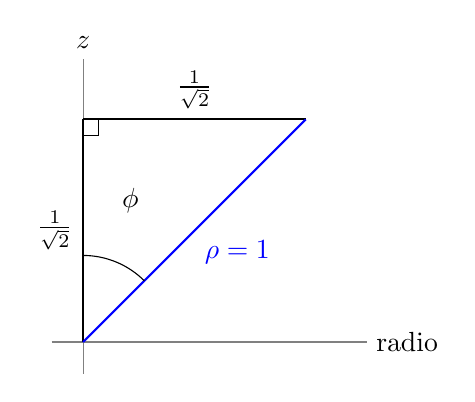
\begin{tikzpicture}[scale=4]
        % Coordenadas
        \coordinate (O) at (0,0); 
        \coordinate (A) at (0,{1/sqrt(2)}); 
        \coordinate (B) at ({1/sqrt(2)},{1/sqrt(2)}); 

        % Ejes tenues
        \draw[gray] (-0.1,0) -- (0.9,0) node[right, black] {radio};
        \draw[gray] (0,-0.1) -- (0,0.9) node[above, black] {$z$};

        % Dibujo del triángulo
        \draw[thick] (O) -- (A) node[midway, left] {$\frac{1}{\sqrt{2}}$}; 
        \draw[thick] (A) -- (B) node[midway, above] {$\frac{1}{\sqrt{2}}$}; 
        \draw[thick, blue] (O) -- (B) node[midway, below right] {$\rho=1$}; 

        % Ángulo recto
        \draw (A) ++(0,-0.05) -- ++(0.05,0) -- ++(0,0.05);

        % Arco de phi interno (Solucionado: dibujado a mano sin depender de librerías)
        \draw (0, 0.275) arc (90:45:0.275);
        \node at (0.15, 0.45) {$\phi$};
    \end{tikzpicture}
